\documentclass[10pt, aspectratio=169]{beamer}

\usetheme[progressbar=frametitle, sectionpage=progressbar, subsectionpage=progressbar, numbering=fraction, block=fill]{metropolis}

\definecolor{mLightBrown}{HTML}{4D4D4D}
\definecolor{mMediumBrown}{HTML}{2C2C2A}
\definecolor{mDarkBrown}{HTML}{1A1A19}
\definecolor{mDarkTeal}{HTML}{0F6E56}
\definecolor{mDarkRed}{HTML}{B03A2E}
\setbeamercolor{normal text}{fg=mDarkBrown}
\setbeamercolor{alerted text}{fg=mDarkTeal}
\setbeamercolor{frametitle}{bg=mDarkBrown}
\setbeamercolor{progress bar}{fg=mDarkTeal, bg=mDarkTeal!20}
\definecolor{mPaleBg}{HTML}{F4F3EE}
\setbeamercolor{block title}{bg=mDarkBrown!10, fg=mDarkBrown}
\setbeamercolor{block body}{bg=mPaleBg, fg=mDarkBrown}
\newcommand{\hl}[1]{\textcolor{mDarkTeal}{#1}}

\usepackage{amsmath, amssymb, amsthm, mathtools}
\usepackage{cancel}\usepackage{bm}\usepackage{booktabs}\usepackage{array}
\usepackage{xcolor}\usepackage{colortbl}\usepackage{multirow}\usepackage{tikz}
\usetikzlibrary{positioning,arrows.meta,calc,fit,shapes.geometric,decorations.pathmorphing}

\newcommand{\paper}[1]{\textcolor{mLightBrown}{\small\textit{(#1)}}}

\newcommand{\qcur}{0}
\newcommand{\qnode}[4]{%
\ifnum#4=\qcur
 \node[draw=mDarkTeal, fill=mDarkTeal!12, thick, rounded corners=1pt, minimum width=3.0cm, minimum height=0.52cm, font=\tiny\bfseries, text=mDarkBrown] (#2) at (#1,0) {#3};%
\else
 \node[draw=mLightBrown!45, rounded corners=1pt, minimum width=3.0cm, minimum height=0.52cm, font=\tiny, text=mLightBrown] (#2) at (#1,0) {#3};%
\fi}
\newcommand{\qstrip}[1]{\renewcommand{\qcur}{#1}%
\begin{center}
\begin{tikzpicture}
\qnode{0}{q1}{Q1 Formulate?}{1}
\qnode{3.7}{q2}{Q2 Convex?}{2}
\qnode{7.4}{q3}{Q3 Certify?}{3}
\qnode{11.1}{q4}{Q4 Hard ones?}{4}
\draw[-{Stealth}, mLightBrown!60] (q1.east) -- (q2.west);
\draw[-{Stealth}, mLightBrown!60] (q2.east) -- (q3.west);
\draw[-{Stealth}, mLightBrown!60] (q3.east) -- (q4.west);
\end{tikzpicture}\end{center}}

\title{Optimization Problem Modeling}
\subtitle{Before you can learn a decision, you must be able to state one}
\author{Jinkyoo Park}
\institute{KAIST}
\date{\textit{Lecture 1 --- The atom every later method is built from}}

\begin{document}

\maketitle

%==========================================================
\section{The handoff --- the purest decision}
%==========================================================

\begin{frame}{Where we are --- the simplest cell of the map}
\vspace{2pt}
\begin{center}\footnotesize\renewcommand{\arraystretch}{1.5}
\begin{tabular}{r|c|c}
 & \textbf{Model-based} & \textbf{Data-driven} \\
\hline
\textbf{Static, single}  & \cellcolor{mDarkTeal!20}\textbf{optimization} \scriptsize(\alert{Lec.\ 1}) & Bayesian / learned opt.\ \scriptsize(Lec.\ 2--6)\\
\hline
\textbf{Dynamic, single} & MDP \,/\, optimal control \scriptsize(Lec.\ 7, 9) & RL \scriptsize(Lec.\ 8, 10, 11)\\
\end{tabular}
\end{center}
\smallskip

We begin at the \alert{simplest cell}: one decision, a known objective, no time, no rivals. This is classical mathematical optimization.
\smallskip

\pause
Why start here when the course is about \emph{data-driven} decisions? Because this is the \alert{atom}. Every later method --- Bayesian optimization, value iteration, policy gradient, trust-region RL --- is this template with something made uncertain, sequential, or sampled. Master the atom and the molecules become legible.
\end{frame}

\begin{frame}{The thesis --- formulation precedes solution}
The fixed point of this lecture, in one line:
\begin{center}\large
\alert{Before you can learn a decision, you must be able to state one.}
\end{center}
\medskip

\pause
A decision problem becomes mathematics through three ingredients --- and naming them is half the work:
\begin{itemize}\setlength\itemsep{2pt}
\item an \textbf{objective} $f(x)$ --- what ``good'' means, as a number to minimize;
\item \textbf{decision variables} $x$ --- the levers you may pull;
\item \textbf{constraints} $g(x)\le0,\ h(x)=0$ --- what is allowed.
\end{itemize}
\medskip

\pause
Get this right and the rest is method. Get it wrong --- the wrong objective, a missing constraint --- and no solver, classical or learned, can save you. The hardest, most consequential step in applied decision-making is the \alert{modeling}, not the solving.
\end{frame}

\begin{frame}{The roadmap --- four questions}
\qstrip{0}
\medskip
\begin{itemize}\setlength\itemsep{3pt}
\item \textbf{Q1 --- How do we state a decision mathematically?} The \alert{standard form}.
\item \textbf{Q2 --- Which problems can we actually solve?} \alert{Convexity} --- the great watershed.
\item \textbf{Q3 --- How do we \emph{know} a solution is optimal?} Optimality conditions and \alert{KKT}.
\item \textbf{Q4 --- What about the non-convex ones?} \alert{Successive convexification} and trust regions.
\end{itemize}
\end{frame}

%==========================================================
\section{Act 1 --- the standard form}
%==========================================================

\begin{frame}{The standard form --- one shape for all of them}
\qstrip{1}
\medskip
Every mathematical optimization problem can be written:
\[
\min_{x\in D}\; f(x) \qquad \text{s.t.}\quad g_i(x)\le 0,\ i=1,\dots,m, \qquad h_j(x)=0,\ j=1,\dots,p.
\]
\begin{itemize}\setlength\itemsep{1pt}
\item $x\in\mathbb{R}^n$ --- the optimization variable; $f:\mathbb{R}^n\to\mathbb{R}$ --- objective;
\item $g_i$ --- inequality constraints; $h_j$ --- equality constraints;
\item the \alert{optimal value} $p^* = \inf\{f(x): x \text{ feasible}\}$.
\end{itemize}
\medskip

\pause
Two degenerate cases worth naming: $p^*=+\infty$ if the problem is \emph{infeasible} (no $x$ satisfies the constraints), $p^*=-\infty$ if it is \emph{unbounded below}. Both are usually signs of a modeling error, not a solver failure.
\medskip

\pause
{\footnotesize\textcolor{mLightBrown}{Maximizing $f$ is minimizing $-f$; everything is phrased as minimization without loss of generality.}}
\end{frame}

%==========================================================
\section{Act 2 --- convexity, the watershed}
%==========================================================

\begin{frame}{Convexity --- the line between easy and hard}
\qstrip{2}
\medskip
A problem is \alert{convex} when $f$ is a convex function and the feasible set is a convex set ($g_i$ convex, $h_j$ affine).
\medskip

\pause
\begin{block}{Why convexity is \emph{the} dividing line}
\centering
For a convex problem, \alert{any local minimum is a global minimum.}
\end{block}
\medskip

\pause
That single fact changes everything:
\begin{itemize}\setlength\itemsep{1pt}
\item reliable, efficient solvers exist; initialization and step-size do not trap you in bad local optima;
\item global optimality is \alert{certifiable} (via KKT --- Act 3);
\item duality gives a computable lower bound and an optimality gap;
\item the problem decomposes well for distributed / large-scale solving.
\end{itemize}
\medskip
\pause
Non-convex problems enjoy none of these for free. Much of practical optimization is the art of \alert{getting a convex problem} --- or a sequence of them.
\end{frame}

\begin{frame}{The convex family --- LP, QP, QCQP}
Named convex forms, in order of generality:
\medskip
\begin{center}\footnotesize\renewcommand{\arraystretch}{1.5}
\begin{tabular}{l|l|l}
\textbf{Class} & \textbf{Objective} & \textbf{Feasible set} \\
\hline
\textbf{Linear program (LP)} & $c^\top x + d$ & polyhedron (affine ineq.) \\
\textbf{Quadratic program (QP)} & $\tfrac12 x^\top P x + q^\top x$, $P\succeq0$ & polyhedron \\
\textbf{QCQP} & convex quadratic & intersection of ellipsoids \\
\end{tabular}
\end{center}
\medskip

\pause
The progression matters because modeling is often a matter of \emph{recognizing} which named class your problem (or its convexified version) falls into --- each has mature, reliable solvers. The LP's optimum sits at a vertex of the polyhedron; the QP's, where the quadratic's level sets first touch the feasible region.
\medskip

\pause
{\footnotesize\textcolor{mLightBrown}{These same quadratic models reappear in Act 4 as the \emph{local} approximation of hard problems --- and, much later, as the trust-region subproblem inside TRPO (Lecture 10).}}
\end{frame}

%==========================================================
\section{Act 3 --- certifying optimality}
%==========================================================

\begin{frame}{When is a point optimal? --- the first-order condition}
\qstrip{3}
\medskip
For a convex problem $\min_{x\in D} f(x)$ with differentiable $f$, a feasible $x^*$ is optimal \emph{iff}
\[
\nabla f(x^*)^\top (y - x^*) \ge 0 \quad \text{for all feasible } y.
\]
\medskip

\pause
\textbf{Reading it geometrically.} Moving from $x^*$ toward any other feasible point cannot decrease $f$ --- there is no improving feasible direction. If $\nabla f(x^*)\ne0$, it defines a \alert{supporting hyperplane} to the feasible set at $x^*$: the whole feasible region lies on the ``uphill'' side.
\medskip

\pause
\begin{center}\large
Optimality $=$ no feasible direction points downhill.
\end{center}
For an \emph{unconstrained} convex problem this collapses to the familiar $\nabla f(x^*) = 0$.
\end{frame}

\begin{frame}{KKT --- optimality with constraints, and a dual bound}
With constraints, introduce multipliers $\lambda_i\ge0$ (for $g_i$) and $\nu_j$ (for $h_j$). The \alert{Karush--Kuhn--Tucker} conditions characterize optimality:
\[
\nabla f(x^*) + \sum_i \lambda_i \nabla g_i(x^*) + \sum_j \nu_j \nabla h_j(x^*) = 0, \quad
g_i(x^*)\le0,\ h_j(x^*)=0,\ \lambda_i\ge0,\ \lambda_i g_i(x^*)=0.
\]
\medskip

\pause
The last identity, \alert{complementary slackness}, says each constraint is either active ($g_i=0$) or ignored ($\lambda_i=0$). For convex problems, KKT is \emph{necessary and sufficient} --- a certificate of global optimality.
\medskip

\pause
\textbf{Duality, in one line.} The Lagrangian $L(x,\lambda,\nu)=f(x)+\sum_i\lambda_i g_i+\sum_j\nu_j h_j$ yields a dual function whose value \alert{lower-bounds} $p^*$ for any $\lambda\ge0$. The gap between primal and dual is a computable measure of how close you are.
\medskip
\pause
{\footnotesize\textcolor{mLightBrown}{Differentiating the KKT system is exactly how one back-propagates through an optimization layer --- the trick behind differentiable LQR/MPC in Lecture 11.}}
\end{frame}

%==========================================================
\section{Act 4 --- when the problem is not convex}
%==========================================================

\begin{frame}{Successive convexification --- solve a sequence of easy problems}
\qstrip{4}
\medskip
Real engineering problems are usually non-convex (non-convex objective, non-convex constraints). The dominant strategy: \alert{don't solve the hard problem --- solve a sequence of convex approximations to it.}
\medskip

\pause
At the current iterate $x^{(k)}$, build a local convex model:
\[
\tilde f(x) = f(x^{(k)}) + \nabla f(x^{(k)})^\top (x - x^{(k)}) + \tfrac12 (x-x^{(k)})^\top B^{(k)} (x-x^{(k)}),
\]
linearize the awkward constraints, and add a \alert{trust region} $\|x - x^{(k)}\| \le \rho^{(k)}$ so the model stays trustworthy.
\medskip

\pause
\begin{center}\large
The trust region is the key idea: \alert{only trust the approximation nearby.}
\end{center}
Solve the convex subproblem; if it improves the true objective, accept and \emph{grow} $\rho$; if not, reject and \emph{shrink} $\rho$. Repeat.
\end{frame}

\begin{frame}{Case study --- wind-farm layout optimization}
Place $N$ turbines to maximize power, subject to minimum inter-turbine spacing and boundary constraints --- a non-convex problem (the spacing constraints are non-convex).
\medskip
\begin{center}
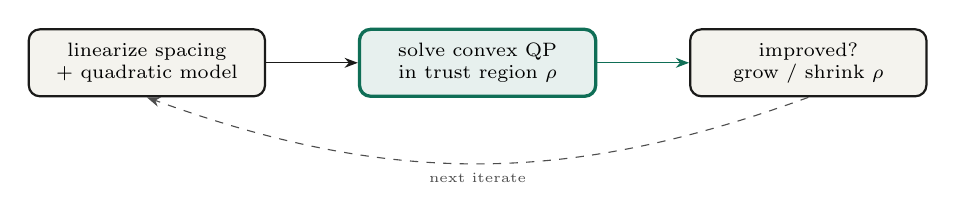
\begin{tikzpicture}[font=\scriptsize, node distance=4pt]
\node[draw=mDarkBrown, thick, fill=mPaleBg, rounded corners, minimum width=3.0cm, minimum height=0.85cm, align=center] (a) at (0,0) {linearize spacing\\ + quadratic model};
\node[draw=mDarkTeal, very thick, fill=mDarkTeal!10, rounded corners, minimum width=3.0cm, minimum height=0.85cm, align=center] (b) at (4.2,0) {solve convex QP\\ in trust region $\rho$};
\node[draw=mDarkBrown, thick, fill=mPaleBg, rounded corners, minimum width=3.0cm, minimum height=0.85cm, align=center] (c) at (8.4,0) {improved?\\ grow / shrink $\rho$};
\draw[-{Stealth}, mDarkBrown] (a) -- (b);
\draw[-{Stealth}, mDarkTeal] (b) -- (c);
\draw[-{Stealth}, mLightBrown, dashed] (c.south) to[bend left=20] node[below,font=\tiny]{next iterate} (a.south);
\end{tikzpicture}
\end{center}
\medskip

\pause
Each iteration is a convex QP (solved reliably); the trust region guarantees the linearized constraints stay close to the true ones. The non-convex layout problem is conquered by \alert{a staircase of convex problems} --- the practical face of Act 2's lesson: \emph{get a convex problem, even if you have to keep making new ones}.
\end{frame}

%==========================================================
\section{Closing}
%==========================================================

\begin{frame}{Where we are --- and the assumption we now drop}
\vspace{2pt}
\begin{center}\footnotesize\renewcommand{\arraystretch}{1.5}
\begin{tabular}{r|c|c}
 & \textbf{Model-based} & \textbf{Data-driven} \\
\hline
\textbf{Static, single}  & \cellcolor{mDarkTeal!15}\textbf{optimization} \;{\scriptsize Lec.\ 1 \checkmark} & Bayesian / learned opt.\ \;{\scriptsize Lec.\ 2--6 $\to$}\\
\end{tabular}
\end{center}
\medskip

\pause
We can now \emph{state} a decision and, when it is convex (or convexifiable), \emph{solve and certify} it. But every line above assumed one thing:
\begin{center}\large
\alert{the objective $f$ and constraints were known, exactly.}
\end{center}
\medskip

\pause
What if $f$ has \emph{uncertain parameters} --- a model fit to noisy data? Then a single best $x$ is not enough; we must reason about our \alert{uncertainty} about $f$ itself. That is Lecture 2: don't pick a number --- carry a belief.
\end{frame}

\begin{frame}{Closing --- the one sentence}
\vfill
\begin{center}\large
Optimization is how a decision becomes mathematics ---\\[8pt]
an objective to minimize, levers to pull, limits to respect ---\\[4pt]
and, when the problem is convex,\\[4pt]
an answer we can not only find but \alert{prove}.
\end{center}
\vfill
\pause
\footnotesize
Hold onto two pieces: the standard form (it is the skeleton of every objective to come) and the trust region (it returns in surrogate optimization and again in trust-region RL). Everything else this term is this atom, perturbed by uncertainty.
\end{frame}

\begin{frame}[standout]
Questions?
\end{frame}

%==========================================================
\appendix
%==========================================================

\begin{frame}{Backup 1 --- KKT conditions in full}
\footnotesize
For $\min f(x)$ s.t.\ $g_i(x)\le0$, $h_j(x)=0$, the KKT conditions at $x^*$ (with multipliers $\lambda^*\ge0$, $\nu^*$):
\begin{itemize}\setlength\itemsep{1pt}
\item \textbf{Stationarity:} $\nabla f(x^*) + \sum_i \lambda_i^* \nabla g_i(x^*) + \sum_j \nu_j^* \nabla h_j(x^*) = 0$;
\item \textbf{Primal feasibility:} $g_i(x^*)\le0$, $h_j(x^*)=0$;
\item \textbf{Dual feasibility:} $\lambda_i^*\ge0$;
\item \textbf{Complementary slackness:} $\lambda_i^*\, g_i(x^*) = 0$.
\end{itemize}
\medskip
\textbf{Convex case.} If $f,g_i$ are convex and $h_j$ affine (and a constraint qualification such as Slater's holds), KKT is \emph{necessary and sufficient} for global optimality --- a checkable certificate. \textbf{Non-convex case.} KKT remains necessary (under a constraint qualification) but not sufficient: a KKT point may be a local min, saddle, or local max.
\end{frame}

\begin{frame}{Backup 2 --- Lagrangian duality and the gap}
\footnotesize
\textbf{Lagrangian.} $L(x,\lambda,\nu) = f(x) + \sum_i \lambda_i g_i(x) + \sum_j \nu_j h_j(x)$.
\medskip

\textbf{Dual function.} $d(\lambda,\nu) = \inf_x L(x,\lambda,\nu)$. For any $\lambda\ge0$ and any $\nu$, weak duality gives $d(\lambda,\nu)\le p^*$ --- the dual is a \emph{lower bound} on the optimum, always.
\medskip

\textbf{Dual problem.} $\max_{\lambda\ge0,\nu} d(\lambda,\nu) =: d^*$. The \alert{duality gap} is $p^* - d^*\ge0$. For convex problems with a constraint qualification, the gap is zero ($p^*=d^*$, \emph{strong duality}) --- so the dual optimum certifies the primal.
\medskip
\textbf{Use.} Even when you cannot solve the primal, evaluating $d(\lambda,\nu)$ at any feasible dual point brackets how far your current solution can possibly be from optimal --- the practical value of duality.
\end{frame}

\begin{frame}{Backup 3 --- the successive convex programming loop}
\footnotesize
\textbf{Algorithm (trust-region SCP).}
\begin{enumerate}\setlength\itemsep{1pt}
\item Initialize $x^{(0)}$, trust radius $\rho^{(0)}$.
\item \textbf{repeat} until $\|x^{(k)} - x^{(k-1)}\| < \epsilon$:
\item \quad form the convex model $\tilde f$ (gradient $+$ approximate Hessian $B^{(k)}$); linearize constraints;
\item \quad solve the convex subproblem over the trust region $\{x: \|x-x^{(k)}\|\le\rho^{(k)}\}$ $\to$ candidate $\tilde x$;
\item \quad compute the ratio $r = \dfrac{f(x^{(k)}) - f(\tilde x)}{f(x^{(k)}) - \tilde f(\tilde x)}$ (actual vs.\ predicted improvement);
\item \quad if $r \ge a$: accept $x^{(k+1)} = \tilde x$ and grow $\rho^{(k+1)} = \beta_{\text{succ}}\,\rho^{(k)}$;
\item \quad else: reject $x^{(k+1)} = x^{(k)}$ and shrink $\rho^{(k+1)} = \beta_{\text{fail}}\,\rho^{(k)}$.
\end{enumerate}
\medskip
\textbf{Why the ratio test.} It measures whether the convex model can be trusted at the proposed step. Trust grows where the model predicts well and shrinks where it does not --- the exact logic that, in policy space, becomes TRPO's KL trust region (Lecture 10).
\end{frame}

\end{document}
